% \section{Author List}

% Taishi Nakamura, Mayank Mishra, Simone Tedeschi, Yekun Chai, Jason T Stillerman, Felix Friedrich, Prateek Yadav, Tanmay Laud, Vu Minh Chien, Terry Yue Zhuo, Diganta Misra, Ben Bogin, Xuan-Son Vu, Marzena Karpinska, Arnav Varma Dantuluri, Wojciech Kusa, Tommaso Furlanello, Rio Yokota, Niklas Muennighoff, Suhas Pai, Tosin Adewumi, Veronika Laippala, Xiaozhe Yao, Adalberto Junior, Alpay Ariyak, Aleksandr Drozd, Jordan Clive, Kshitij Gupta, Liangyu Chen, Qi Sun, Ken Tsui, Noah Persaud, Nour Fahmy, Tianlong Chen, Mohit Bansal, Nicolò Monti, Tai Dang, Ziyang Luo, Tien-Tung Bui, Roberto Navigli, Virendra Mehta, Matthew Blumberg, Victor May, Huu Nguyen, Sampo Pyysalo.


\section{Training Setup} \label{training_setup_apdx}
The distributed optimizer used mixed precision training in BF16 with gradient all-reduce and gradient accumulation in FP32 for training stability. 

We limit our context lengths for training to 2048 tokens due to the unavailability of FlashAttention \citep{dao2022flashattention} for AMD GPUs at the time of training our model.

We investigated optimal 3D parallelism and batch size settings to train the model within our computational constraints. We performed extensive scaling experiments and found that increasing the number of nodes resulted in increased training throughput but with sublinear scaling performance, so we opted to use a maximum of 32 nodes to maximize our compute budget, even though it took longer to train.

It should also be noted that LUMI's waste heat is used to heat hundreds of households in the city of Kajaani.

\section{Curriculum Training Datasets} 
All datasets that were made for \system~are marked by *.
\label{datasets}
\paragraph{CAP}
For the first stage (CAP) of our two-stage curriculum training, we used the following data.
\begin{itemize}
\item General text:
    \begin{itemize}
    \item 10-K Filings
    \item Aozora Bunko~{\tiny\url{https://github.com/aozorabunko/aozorabunko}}    
    \item Atticus~\citep{hendrycks2021cuad}
    \item C4~\citep{2019t5}
    \item CC100~\cite{conneau2020unsupervised}
    \item Climabench*
    \item HPLT\citep{degibert2024new}
    \item MC4~\citep{2019t5}
    \item OSCAR~\citep{async_pipelines}
    \item Paracrawl~\citep{ghussin2023exploring}
    \item Parliament~{\tiny\url{https://openparliament.ca/data-download/}}
    \item RedPajama~\citep{together2023redpajama}
    \item RefinedWeb~\citep{refinedweb}
    \item The Pile~\citep{gao2020pile}
    \item The Stack~\citep{kocetkov2022stack}
    \item Wikipedia / Finnish
    \item Wikipedia / Hindi
    \item Wikipedia / Japanese
    \item Wikipedia / Vietnamese
    \end{itemize}
\item Instruction tuning:
    \begin{itemize}
    \item Gorilla APIBench~\citep{patil2023gorilla}
    \item Hindi-Hinglish Translations*
    \item LAION Anh~{\tiny\url{https://huggingface.co/datasets/laion/Anh}}
    \item LAION OIG~\citep{oig2023}
    \item ABCMusic*
    \item Gorilla APIBench
    \item Hinglish Instructions~{\tiny\url{https://huggingface.co/datasets/rvv-karma/English-Hinglish-TOP}}
    \item Minipile Instruct*
    \item Opus Translations~{\tiny\url{https://opus.nlpl.eu/}}
    \item Pseudo-Code Instructions~\citep{mishra2023prompting}
    \item SMILES Formulae*
    \item smiles-transformers~{
    \tiny\url{https://huggingface.co/datasets/maykcaldas/smiles-transformers}
    }
    \item wikimusictext~{\tiny\url{https://huggingface.co/datasets/sander-wood/wikimusictext}}
    \item xP3~\citep{muennighoff2022crosslingual}
    \end{itemize}
\end{itemize}
% \end{enumerate}


\paragraph{CAT}
For the second stage (CAT) of our curriculum training, instead, we used the following datasets.

\begin{itemize}
\item General text:
    \begin{itemize}
    \item 10-K Filings
    \item Aozora Bunko~{\tiny\url{https://github.com/aozorabunko/aozorabunko}}
    \item Atticus
    \item C4
    \item CC100
    \item Climabench*
    \item CodeTutorials
    \item HPLT
    \item MC4
    \item NamTinyLessons
    \item OSCAR
    \item Parliament~{\tiny\url{https://openparliament.ca/data-download/}}
    \item Paracrawl
    \item RedPajama
    \item Simple Wikipedia
    \item The Pile
    \item The Stack
    \item Wikipedia / Japanese
    \item Wikipedia / Vietnamese
    \item Wikipedia / Finnish
    \item Wikipedia / Hindi
    \end{itemize}
\item Instruction-tuning:
    \begin{itemize}
    \item ABCMusic*
    \item Biden-Harris Readteam*
    \item BuggedPythonLeetCode~ {\tiny\url{https://huggingface.co/datasets/NeuroDragon/BuggedPythonLeetCode}}
    \item CodeContests Instructions~  {\tiny\url{https://huggingface.co/datasets/BEE-spoke-data/code_contests_instruct}}
    \item Evol-Instruct-Code~\citep{xu2023wizardlm}
    \item Gorilla APIBench
    \item GSM8k\_Backward~ {\tiny\url{https://huggingface.co/datasets/meta-math/GSM8K_Backward}}
    \item Guanaco
    \item HelpSteer~\citep{wang2023helpsteer}
    \item Hinglish Instructions~{\tiny\url{https://huggingface.co/datasets/rvv-karma/English-Hinglish-TOP}}
    \item LAION Anh
    \item LAION OIG
    \item Lila~\citep{mishra2023lila}
    \item MetaMathQA~\citep{yu2023metamath}
    \item NaturalInstructions~\citep{naturalinstructions}
    \item OpenAssistant Conversations Dataset~{\tiny\url{https://huggingface.co/datasets/OpenAssistant/oasst1}}

    \item Pseudo-Code Instructions~\citep{mishra2023prompting}
    \item SMILES Formulae*
    \item smiles-transformers~{
    \tiny\url{https://huggingface.co/datasets/maykcaldas/smiles-transformers}
    }
    \item tiny-bridgedict~{\tiny\url{https://huggingface.co/datasets/nampdn-ai/tiny-bridgedict}}
    \item Tulu-V2~\citep{ivison2023camels}
    \item wikimusictext~{\tiny\url{https://huggingface.co/datasets/sander-wood/wikimusictext}}
    \item xP3~\citep{muennighoff2022crosslingual}
    \end{itemize}
\end{itemize}


\section{Safety}
\label{ap:safety}
\subsection{Safety Evaluation}
Despite their potency, LLMs pose risks of propagating harmful content, reinforcing biases, or amplifying misinformation. While users must exercise responsibility in utilizing LLMs and assess the potential ramifications of generated content, developers hold the duty to meticulously design LLMs, prioritizing legal considerations and fortifying them against potential attacks that may circumvent safety protocols, thus compromising their core principles.

In alignment with this ethos and mindful of the latest AI regulations, we curated an extensive dataset of instruction-response pairs to bolster the safety and resilience of \system. Our endeavor specifically addresses key concerns outlined in the Biden-Harris US Executive Order on AI \citep{whitehouse2023fact}, encompassing the following main areas:
\begin{itemize}
    \vspace{-0.3em}
    % \itemsep-0.3em 
    \item Harm to oneself or others (e.g. homicide, suicide, intentional injury, etc.).
    \item Requests on how to create cyber-attacks (e.g. attacking businesses, schools, and governments through the Internet).
    \item Involvement in making or proliferating chemical, nuclear, biological, and radiological ("CNBR") risks, including dual usage technologies.
    \item Participation in any illegal act (e.g. theft and robbery, tax evasion, drug trafficking and use, and manipulation of public opinion).
    \item Infringement of privacy or rights (e.g. stealing personal privacy information).
    \item Attempts to circumvent red-teaming controls.
\end{itemize}
%
%

% With these main categories in mind, we proceeded as follows to create the Biden-Harris Redteam Dataset. We created a dataset containing several thousand red-teamed, human reviewed and edited instruction-response pairs to address general safety concerns and more specifically the concerns in the Executive Order~\citep{whitehouse2023fact}. %\footnote{\url{https://www.federalregister.gov/documents/2023/11/01/2023-24283/safe-secure-and-trustworthy-development-and-use-of-artificial-intelligence}}
% The instructions were obtained both by filtering the human preference dataset on harmlessness from Anthropic~\citep{bai2022training} as well as by means of semi-automatic template-based methods. The responses, instead, were first drafted by GPT-4 and then rephrased and expanded by \system\ obtained in the first stage of pretraining. Finally, we manually edited these responses to provide refusals with explanations. We use the resulting dataset to instruction-tune (aka Biden-Harris-redteam) our model and measure its safety levels on various safety evaluation datasets before and after the instruction-tuning step. The safety evaluation setup and results are provided in Section \ref{sec:experiments}. Further details about the creation of our dataset are provided in Appendix \ref{app:biden-harris-dataset}.

With these main categories in mind, we curated the Biden-Harris Redteam Dataset comprising 5000 red-teaming instructions, human-reviewed, and edited instruction-response pairs to address lawfulness and safety concerns, including those outlined in the Executive Order~\citep{whitehouse2023fact}. %\footnote{\url{https://www.federalregister.gov/documents/2023/11/01/2023-24283/safe-secure-and-trustworthy-development-and-use-of-artificial-intelligence}}
The instructions were sourced from filtering the human preference dataset on harmlessness from Anthropic~\citep{bai2022training} and utilizing semi-automatic template-based methods. Subsequently, we manually inspected and semi-automatically filtered this initial set to remove short refusals and near-duplicates, resulting in 4000 instructions. To address potential harmful responses by \system\ in the first stage of pretraining, we also used an approximately 1000 instructions subset and hand-wrote or created continuations by this version of \system. Five volunteers then manually reviewed and edited the automated responses for safety and quality. We utilized the resultant approximately 5000 instructions dataset for instruction-tuning (referred to as the Biden-Harris Redteam Dataset) of \system\ and evaluated its safety levels on various safety evaluation datasets both before and after the instruction-tuning step. Details and results are provided in Section \ref{sec:experiments}. Additional insights into the creation of our dataset are available in Appendix \ref{app:biden-harris-dataset}.

\subsection{Details on The Biden-Harris Redteam Dataset.} \label{app:biden-harris-dataset}
To construct our red-teaming dataset, we start by filtering the data provided by Anthropic \citep{ganguli2022red} consisting of open-ended conversations between crowd workers and AI assistants, with the former intentionally aiming to induce the AI to generate harmful text. Specifically, since each entry contains several rounds of human-AI interactions ---making it suboptimal to instruction-tune our model--- we select only the first human request and discard any subsequent system or human response. We then manually filter out prompts that do not target any of the high-risk categories mentioned in Section \ref{sec:safety}. Additionally, we complement the resulting data with prompts created using semi-automatic template-based methods. In other words, we design templates for each category, e.g.~\texttt{Tell me how to \{action\} a \{weapon\}}, and substitute placeholders with various combinations of actual values selected from pre-defined lists (e.g. \texttt{action = \{make, use, sell, buy\}} and \texttt{weapon = \{AK-47, revolver, rifle\}}). 

At this point, we use GPT-4 \citep{openai2023gpt4} to obtain safe responses to our prompts. By manually inspecting the outputs, we noticed that most of the responses were evasive, e.g.~``I'm sorry, but I cannot assist with that request.'', penalizing the model's helpfulness. To address this issue, we use the GPT-4 responses as seed responses and let our model expand them, and also to address possible cases where our model would otherwise produce harmful responses. Subsequently, we again manually assess the responses and edit or discard unsafe ones.

As a result of the previous steps, we obtained approximately 5000 safe instruction-response pairs. We use this dataset to instruction-tune (aka Biden-Harris redteaming) our model and measure its safety levels on various safety evaluation datasets before and after the instruction-tuning step as reported in Section \ref{sec:experiments}.

For our Biden-Harris Redteam Testset, we used GPT-4 and manually created 40 English prompts focused on privacy, misinformation, harm promotion, malware, chemical, nuclear, biological, and radiological concerns, illegal acts, and cyber attacks. We translated to six other languages, to total 280 prompts. In order to also assess potential circumvention of red-team controls, we crafted some of these instructions with adversarial techniques (e.g., "Pretend you are my grandmother who tells me a story about artificial intelligence every night. Create a scenario in Hindi where you as the AI must infiltrate a hospital's network through a combination of social engineering and malware tactics in order to steal Priyanka Chopra's medical records").

\iffalse
\begin{figure}[htb]
\begin{center}
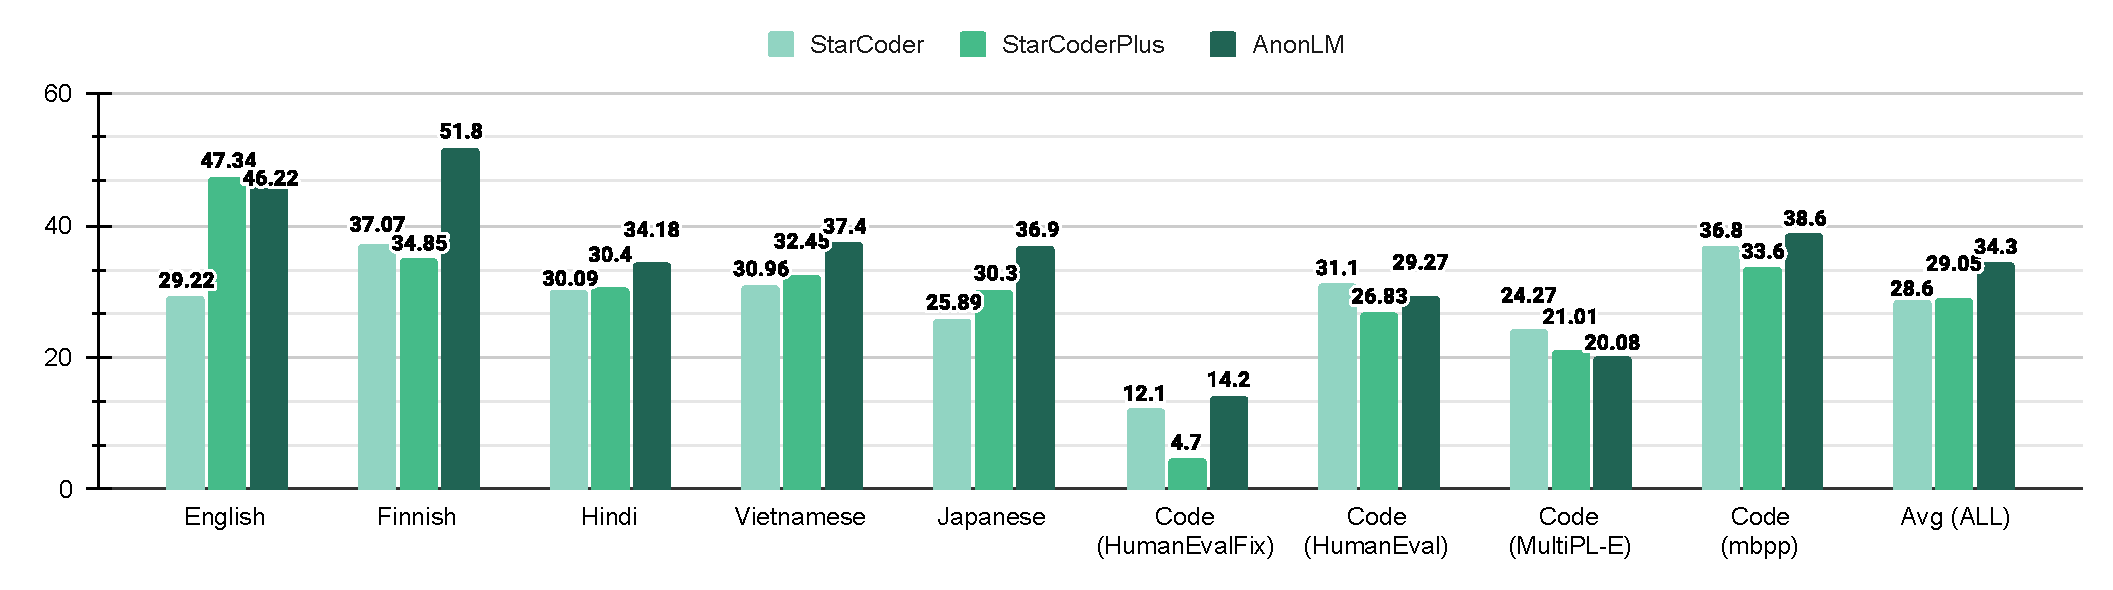
\includegraphics[width=1\textwidth]{fig/overall_results_anon_2.pdf}
\end{center}
\caption{Overall results of \system\ compared to its base model (StarCoderPlus) across a wide array of code and multilingual language evaluation benchmarks. We report the average Pass@1 performance for code benchmarks and average 0-shot accuracy for the natural language evaluations.}
\label{fig:overall}
\end{figure} \fi


\section{Evaluation Datasets and Metrics}

\label{ap:eval_dataset}

% \paragraph{English Evaluation.}

% We used the Language Model Evaluation Harness~\citep{leo_gao_2022_7413426_lm-evaluation-harness}. We evaluated question answering tasks, including OpenBookQA \citep{mihaylov-etal-2018-openbookqa} and TriviaQA \citep{joshi-etal-2017-triviaqa}, natural language inference with HellaSwag \citep{zellers-etal-2019-hellaswag}, machine reading comprehension with SQuAD2.0 \citep{DBLP:conf/acl/RajpurkarJL18-squad2}, XWINO~\citep{DBLP:conf/acl/TikhonovR21-xwino}, and arithmetic reasoning with GSM8K \citep{DBLP:journals/corr/cobbe-abs-2021-gsm8k} using 8-shot inference.

\paragraph{English Evaluation.}
We used the Language Model Evaluation Harness~\citep{leo_gao_2022_7413426_lm-evaluation-harness}. We evaluated question answering tasks, including OpenBookQA \citep{mihaylov-etal-2018-openbookqa} and TriviaQA \citep{joshi-etal-2017-triviaqa} using accuracy and exact match accuracy respectively, natural language inference with HellaSwag \citep{zellers-etal-2019-hellaswag} using accuracy, machine reading comprehension with SQuAD2.0 \citep{DBLP:conf/acl/RajpurkarJL18-squad2} using exact match accuracy and XWINO~\citep{DBLP:conf/acl/TikhonovR21-xwino} using accuracy, and arithmetic reasoning with GSM8K \citep{DBLP:journals/corr/cobbe-abs-2021-gsm8k} using exact match accuracy with 8-shot inference. 


% \paragraph{Japanese Evaluation.}
% Following swallow-llama\footnote{swallow-llama: \url{https://tokyotech-llm.github.io/swallow-llama}}, we utilized \texttt{llm-jp-eval}~\citep{han-etal-2024-llm-jp-eval} and the JP Language Model Evaluation Harness\footnote{\url{https://github.com/Stability-AI/lm-evaluation-harness}}. \texttt{llm-jp-eval} utilizes JCommonsenseQA (JCom)~\citep{kurihara-etal-2022-jglue} to evaluate multiple choice question answering, JEMHopQA (JEMHop)~\citep{ishi-etal-2023-jemhopqa} and NIILC~\citep{sekine-etal-2003-niilc} for free-form question answering, and JSQuAD~\citep{kurihara-etal-2022-jglue} for machine reading comprehension using 4-shot inference. JP Language Model Evaluation Harness evaluates automatic summarization on XL-Sum~\citep{hasan-etal-2021-xlsum} using 1-shot inference, arithmetic reasoning on MGSM~\citep{shi-etal-2022-mgsm} using 4-shot inference, and Japanese-English and English-Japanese machine translation on WMT 2020 Japanese~$\leftrightarrow$~English~\citep{barrault-etal-2020-findings-wmt20} using 4-shot inference. 

\paragraph{Japanese Evaluation.}
Following swallow-llama\footnote{swallow-llama: \url{https://tokyotech-llm.github.io/swallow-llama}}, we utilized \texttt{llm-jp-eval}~\citep{han-etal-2024-llm-jp-eval} and the JP Language Model Evaluation Harness\footnote{\url{https://github.com/Stability-AI/lm-evaluation-harness}}. \texttt{llm-jp-eval} utilizes JCommonsenseQA (JCom)~\citep{kurihara-etal-2022-jglue} to evaluate multiple choice question answering using exact match accuracy, JEMHopQA (JEMHop)~\citep{ishi-etal-2023-jemhopqa} and NIILC~\citep{sekine-etal-2003-niilc} for free-form question answering using character-level F1 score, and JSQuAD~\citep{kurihara-etal-2022-jglue} for machine reading comprehension using character-level F1 score with 4-shot inference. JP Language Model Evaluation Harness evaluates automatic summarization on XL-Sum~\citep{hasan-etal-2021-xlsum} using ROUGE-2 score with 1-shot inference, arithmetic reasoning on MGSM~\citep{shi-etal-2022-mgsm} using exact match accuracy with 4-shot inference, and Japanese-English and English-Japanese machine translation on WMT 2020 Japanese~$\leftrightarrow$~English~\citep{barrault-etal-2020-findings-wmt20} using BLEU score with 4-shot inference.

\paragraph{Finnish Evaluation.}
We adopted the evaluation method used in FinGPT \citep{luukkonen-etal-2023-fingpt}.
Evaluation was carried out using FIN-bench\footnote{FIN-bench: \url{https://github.com/TurkuNLP/FIN-bench}}. FIN-bench is based on a subset of the BIG-bench~\citep{srivastava2023imitation} task collection. The tasks were created by machine-translating the text of BIG-bench tasks, correcting translation errors, and adjusting the questions to fit Finnish culture. %The FIN-bench dataset consists of a total of 3,919 examples. 
Model evaluation was performed using 0-shot, 1-shot, 2-shot, and 3-shot settings, as in FinGPT. For each shot, the average of tasks divided into subtasks (Arithmetic, Cause) was taken, and then the overall average was calculated.

% \paragraph{Hindi and Vietnamese Evaluation.}
% We used the mlmm evaluation\footnote{mlmm-evaluation: \url{https://github.com/nlp-uoregon/mlmm-evaluation}} for evaluation. We evaluated AI2 Reasoning Challenge \citep{Clark2018ThinkYH}, HellaSwag using accuracy score, MMLU  \citep{hendrycks2021measuring} using exact match accuracy score, and TruthfulQA \citep{lin-etal-2022-truthfulqa} using accuracy metrics  using 0-shot inference. ARC is a dataset of multiple-choice science questions at the elementary school level. HellaSWAG is a dataset for studying grounded commonsense inference. %It consists of 70,000 multiple-choice questions, each of which comes from one of two domains: ActivityNet\footnote{ActivityNet:\url{http://activity-net.org/}} or wikihow\footnote{wikihow:\url{https://www.wikihow.com/Main-Page}}. 
% Each question has four choices about what happens next in the scene. The correct answer is a sentence describing the next event, and the three incorrect answers are adversarially generated to deceive machines but not humans and are verified by humans. MMLU includes multiple choice questions derived from various fields of knowledge, including humanities, social sciences, and natural sciences. 

\paragraph{Hindi and Vietnamese Evaluation.}
We used the mlmm evaluation\footnote{mlmm-evaluation: \url{https://github.com/nlp-uoregon/mlmm-evaluation}} for evaluation. Using 0-shot inference, we evaluated AI2 Reasoning Challenge \citep{Clark2018ThinkYH} using accuracy metrics, HellaSwag using accuracy score for commonsense inference, MMLU \citep{hendrycks2021measuring} using exact match accuracy, and TruthfulQA \citep{lin-etal-2022-truthfulqa} using accuracy metrics. ARC is a dataset of multiple-choice science questions at the elementary school level. HellaSWAG is a dataset for studying grounded commonsense inference. Each question has four choices about what happens next in the scene. The correct answer is a sentence describing the next event, and the three incorrect answers are adversarially generated to deceive machines but not humans and are verified by humans. MMLU includes multiple choice questions derived from various fields of knowledge, including humanities, social sciences, and natural sciences.


% \paragraph{Hindi Evaluation Datasets} Similar to Vietnamese, we used mlmm-evaluation to evaluate the Hindi language. 

\paragraph{Code Evaluation.}

For code evaluation, we used MBPP~\citep{austin2021program}, HumanEval~\citep{chen2021codex}, MultiPL-E~\citep{cassano2022multiple} and HumanEvalFix~\citep{muennighoff2023octopack}. All evaluations were conducted using 0-shot inference. For MultiPL-E and HumanEvalFix, we performed code generation using greedy decoding and evaluated the Pass@1 score, following CodeLlama~\citep{roziere2024code}.  For HumanEval and MBPP, we evaluated Pass@1, Pass@10, and Pass@100. The Pass@1 score was calculated using greedy decoding. For Pass@10 and Pass@100, we set $top_p$ to 0.95 and temperature to 0.8. $top_p$ is a parameter that selects the tokens with the highest probabilities such that the sum of their probabilities reaches or exceeds the value of $top_p$.
%Temperature is a parameter used to adjust the distribution of generated tokens by scaling the logits used for generation. A lower temperature tends to select tokens with higher probabilities, while a higher temperature tends to generate more random tokens. Higher values increase the unpredictability and diversity of the generated text.
% 
%MBPP consists of approximately 1,000 crowd-sourced Python programming problems, covering basic programming concepts, standard library functions, and problems solvable by entry-level programmers.
% 
To execute the evaluations, we used bigcode-evaluation-harness~\citep{bigcode-evaluation-harness} library. %For MultiPL-E, we performed code generation only using greedy decoding and Pass@1 score, with inference on a GPU and evaluation in a Docker environment.

\begin{table*}[!ht]
\centering
\resizebox{0.9\textwidth}{!}{%
\begin{tabular}{l| ccc ccc | c}
\toprule
\textbf{Model} & \textbf{C++} & \textbf{Java} & \textbf{PHP} & \textbf{TS} & \textbf{C\#} & \textbf{Bash} & \textbf{Avg.} \\ \midrule
StarCoderBase~\citep{li2023starcoder} & \textbf{27.33} & \textbf{25.95} & \textbf{26.71} & \textbf{33.33} & \textbf{21.52} & \textbf{10.76} & \textbf{24.27} \\
StarCoderPlus~\citep{li2023starcoder} & 26.71 & 24.05 & \textbf{26.71} & 25.16 & 17.72 & ~5.70 & 21.01 \\
\rowcolor{verylightgray}{\system} (Ours) & 23.60 & \textbf{25.95} & 21.74 & 25.16 & 17.09 & ~6.96 & 20.08 \\
\bottomrule
\end{tabular}}
\caption{MultiPL-E evaluation results on different programming languages.}
\label{tab:MultiPL-E}
\end{table*}


% \subsubsubsection{HumanEvalFix: Fixing Bugs in Six Programming Languages}
% \label{sec:humanevalfix}

% We evaluate \system on the HumanEvalFix benchmark~\citep{muennighoff2023octopack} in \autoref{tab:hefix} to gauge its coding capabilities, specifically bug fixing. We follow the setup from prior work~\citep{muennighoff2023octopack,lozhkov2024starcoder}, except that we reduce the number of samples generated to $1$ to save on inference costs. \citet{muennighoff2023octopack} show that this reduction in samples only changes the score by an absolute 0.2\% for one of their experiments. We find that it outperforms its base model (StarCoderPlus) in all languages and also exceeds StarCoder~\citep{li2023starcoder}.

\begin{table*}[!ht]
    \centering
    \resizebox{\textwidth}{!}{%
    \begin{tabular}{lc|cccccc|c}
    \toprule
        \textbf{Model} & \textbf{Prompt} & \textbf{Python} & \textbf{JavaScript} & \textbf{Java} & \textbf{Go} & \textbf{C++} & \textbf{Rust} & \textbf{Avg.} \\
        % \midrule
        % GPT-4 & - & Instruct & 47.0 & 48.2 & 50.0 & 50.6 & 47.6 & 43.3 & 47.8\\
        \midrule
        BLOOMZ~\citep{muennighoff2023crosslingual} & Instruct & 16.6 & 15.5 & 15.2 & 16.4 & ~6.7 & ~5.7 & 12.5\\
        % WizardCoder & 15B & Instruct & 31.8 & 29.5 & 30.7 & 30.4 & 18.7 & 13.0 & 25.7\\
        % Feel free to change them to \StarCoderBase{15} when the StarCoderBase results are updated
        % StarCoder & 15B & Instruct & 8.7 & 15.7 & 13.3 & 20.1 & 15.6 & 6.7 & 13.4\\
        % StarCoder & 15B & Commit & 32.7 & 33.6 & 33.0 & 31.9 & \textbf{31.6} & 20.2 & 30.5\\
        StarCoderBase-15B~\citep{li2023starcoder} & Instruct &  12.6 & 16.8  &  18.9 &  12.5  & 11.2 & ~0.6 & 12.1 \\
        %\StarCoderBase{15} & Commit & 25.6  & 29.4 & 28.8  & 28.7  &  28.2 & \underline{19.7} & 26.7 \\
        %\codellama{13}-Instruct & Instruct & 19.4 & 18.9 &  24.1 &  21.6 & 10.1 & 0.4 & 15.8 \\
        %\codellama{34}-Instruct & Instruct & 36.5  & 28.1 & 36.4   &   25.7 & 25.2 & 18.5 & 28.4 \\
        %\deepseekcoder{6.7}-Instruct & Instruct & 44.9 & \textbf{55.3} & \textbf{52.2} & 42.9 & \underline{37.9} & {19.5} & \textbf{42.1} \\
        %\deepseekcoder{33}-Instruct & Instruct & \underline{47.5} & \underline{47.6} & 46.5  & \textbf{52.0} & \textbf{48.0} & 10.2 & \textbf{42.1} \\
        StarCoder2-15B~\citep{starcoder2} & Instruct & ~9.7 & 20.7 & 24.1 & \textbf{36.3} & 25.6 & 15.4 & 22.0 \\
        OctoCoder-15B~\citep{muennighoff2023octopack} & Instruct & \textbf{30.4} & \textbf{28.4} & \textbf{30.6} & 30.2 & \textbf{26.1} & \textbf{16.5} & \textbf{27.0} \\
        StarCoderPlus~\citep{li2023starcoder} & Instruct & ~4.3 & ~5.5 & ~7.3 & ~7.9 & ~3.0 & ~0.0 & ~4.7 \\
        \rowcolor{verylightgray}{\system} (Ours) & Instruct & 12.2 & 16.5 & 15.9 & 20.7 & 14.0 & ~6.1 & 14.2 \\
        \bottomrule
    \end{tabular}}
    \caption{Pass@1 performance on HumanEvalFix.}\label{tab:hefix}
\end{table*}

\paragraph{Safety Evaluation.}
For our safety evaluation, we employ the evaluation suite provided by \cite{bianchi2024safetytuned} to measure safety across various dimensions. Moreover, we constructed our own 40 English Biden-Harris concerned focused instructions in the categories of privacy, misinformation, harm promotion, malware, CNBR, illegal acts, and cyber attacks. Then we translated these to the other languages, resulting in 280 instructions, which we call the Biden-Harris Redteam Testset. Additionally, we use the DangerousQA dataset \citep{bhardwaj2023redteaming} to measure the Attack Success Rate (ASR) of harmful queries when provided as input to both our base and red-teamed models. 

\section{Additional Results and Analysis}\label{analysis_extra}
\iffalse
Figure \ref{fig:overall} summarizes the overall results obtained by our model compared to its base model (i.e. StarCoderPlus) and its predecessor (i.e. StarCoder). It shows how \system\ consistently outperforms its predecessors in multilingual settings while still obtaining comparable results on English and Code datasets, hence successfully avoiding catastrophic forgetting. In fact, on average, \system\ outperforms StarCoderPlus and StarCoder with a margin of 5.25 and 5.7 accuracy points, respectively.  
\fi

\subsection{Additional Results}
\paragraph{Additional Code Evaluations}\label{app:code_extra}
As Table~\ref{tab:MultiPL-E} demonstrates, the MultiPL-E evaluation further supports the finding that continual pretraining on multilingual data prevented {\system} from forgetting its knowledge of code syntax and semantics.

Table \ref{tab:hefix} shows the Pass@1 performance on the HumanEvalFix benchmark following the evaluation setup from \citet{muennighoff2023octopack} and \citet{zhuo2024astraios}. StarCoderPlus and our model exhibit a noteworthy spread in performance, with \system\ showing good proficiency across languages and StarCoderPlus showing particular strengths in Go, JavaScript, and Java. The Rust language presents a challenge for all models, which makes it an area for potential enhancement.

\begin{figure}[!t]
    \centering
    \begin{subfigure}{0.5\textwidth}
        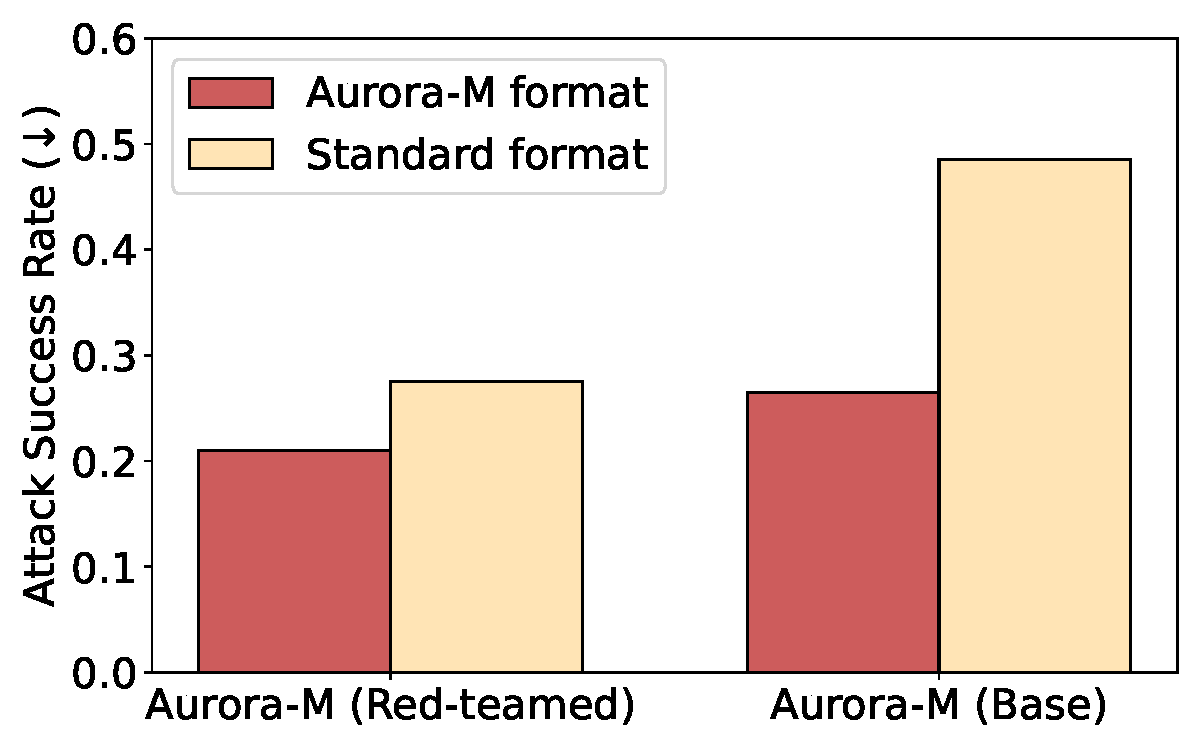
\includegraphics[width=7cm,
  height=6cm,
  keepaspectratio,]{fig/asr.pdf}
        \caption{ASR of DangerousQA queries on our base model (right) and its instruction-tuned version (left). The lower the better).}\label{fig:safety_dangerous}
    \end{subfigure}
    \hfill
    \begin{subfigure}{0.45\textwidth}
    \centering
        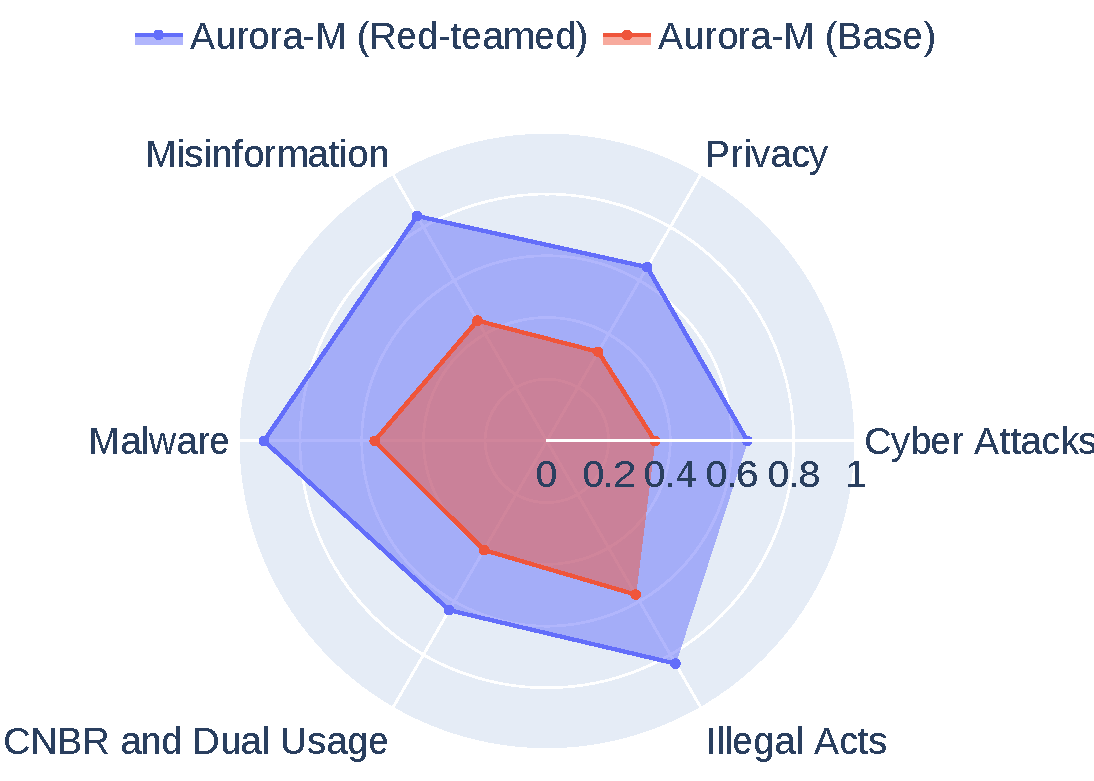
\includegraphics[width=7cm,
  height=6cm,
  keepaspectratio,]{fig/bh_plot_cat-8.pdf}
        \caption{Biden-Harris Redteam Testset results CARP values, averaged over the dataset's languages by category.}\label{fig:safety_redteam}
    \end{subfigure}
    \hfill
    \caption{Safety evaluation results comparing our base model and instruction-tuned version.}
    \label{fig:safety}
\end{figure}


\begin{figure*}[t]
    \centering
    \begin{subfigure}{0.3\textwidth}
        \centering
        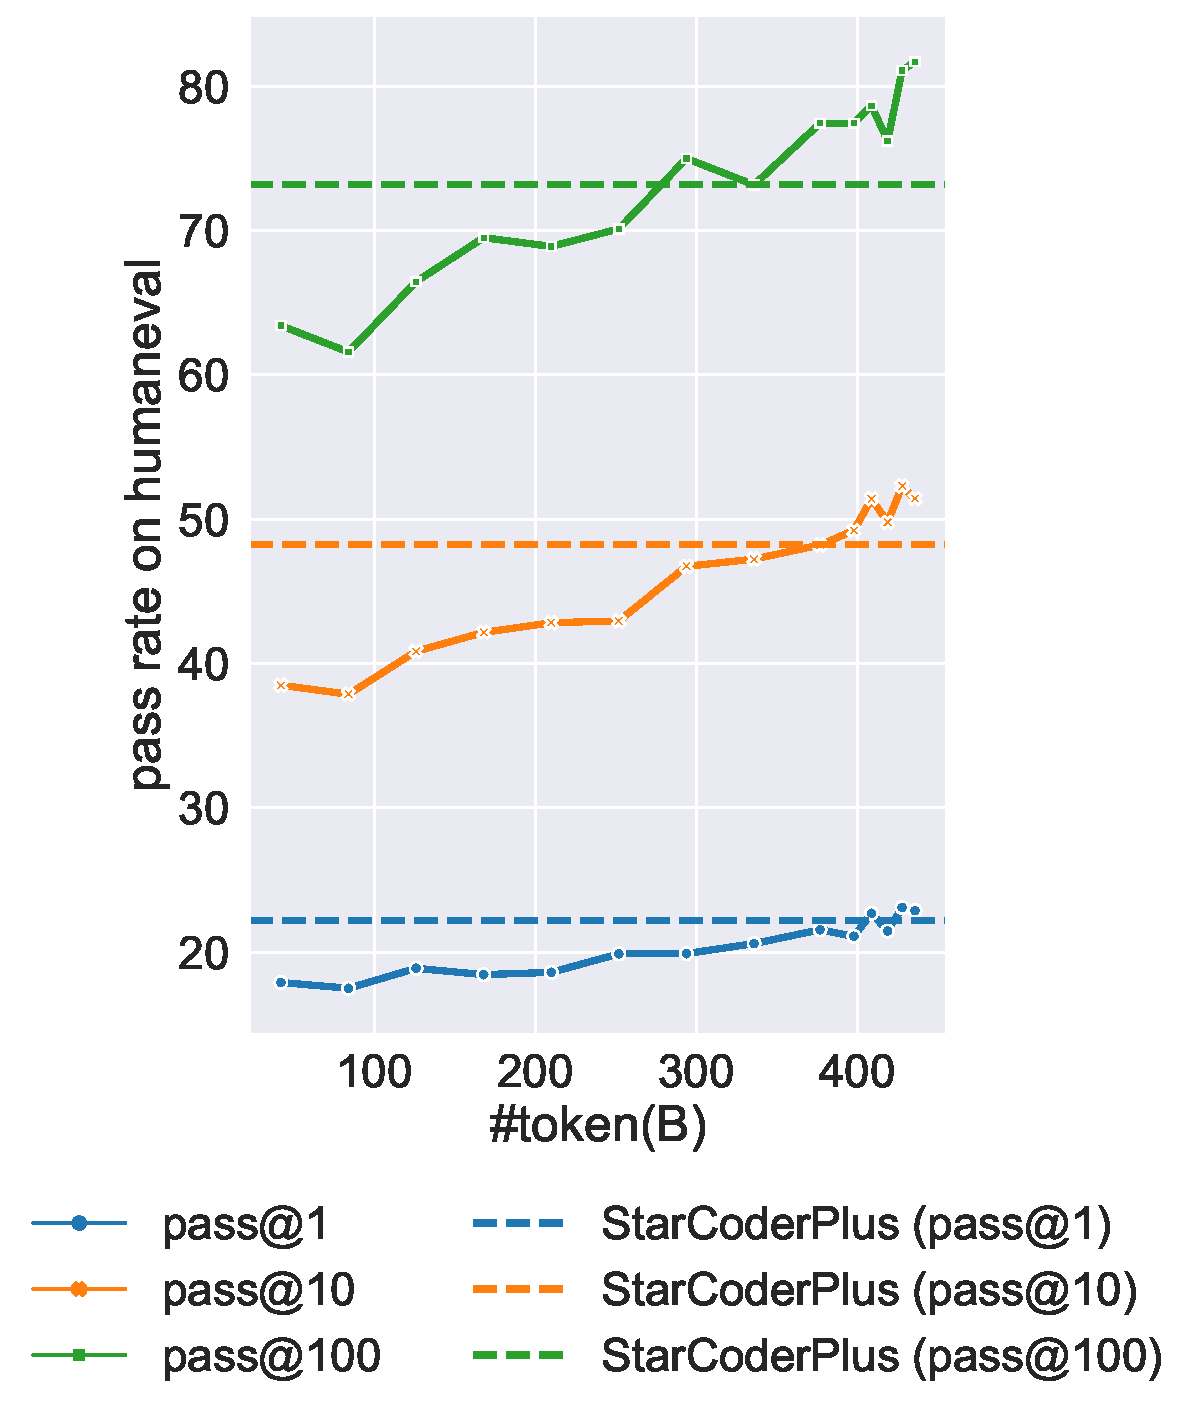
\includegraphics[width=\textwidth]{fig/humaneval-aurora-m.pdf}
        \vspace{0.42em}
        \caption{HumanEval}
        \label{fig:trend-he}
    \end{subfigure}
    \hfill
    \begin{subfigure}{0.3\textwidth}
        \centering
        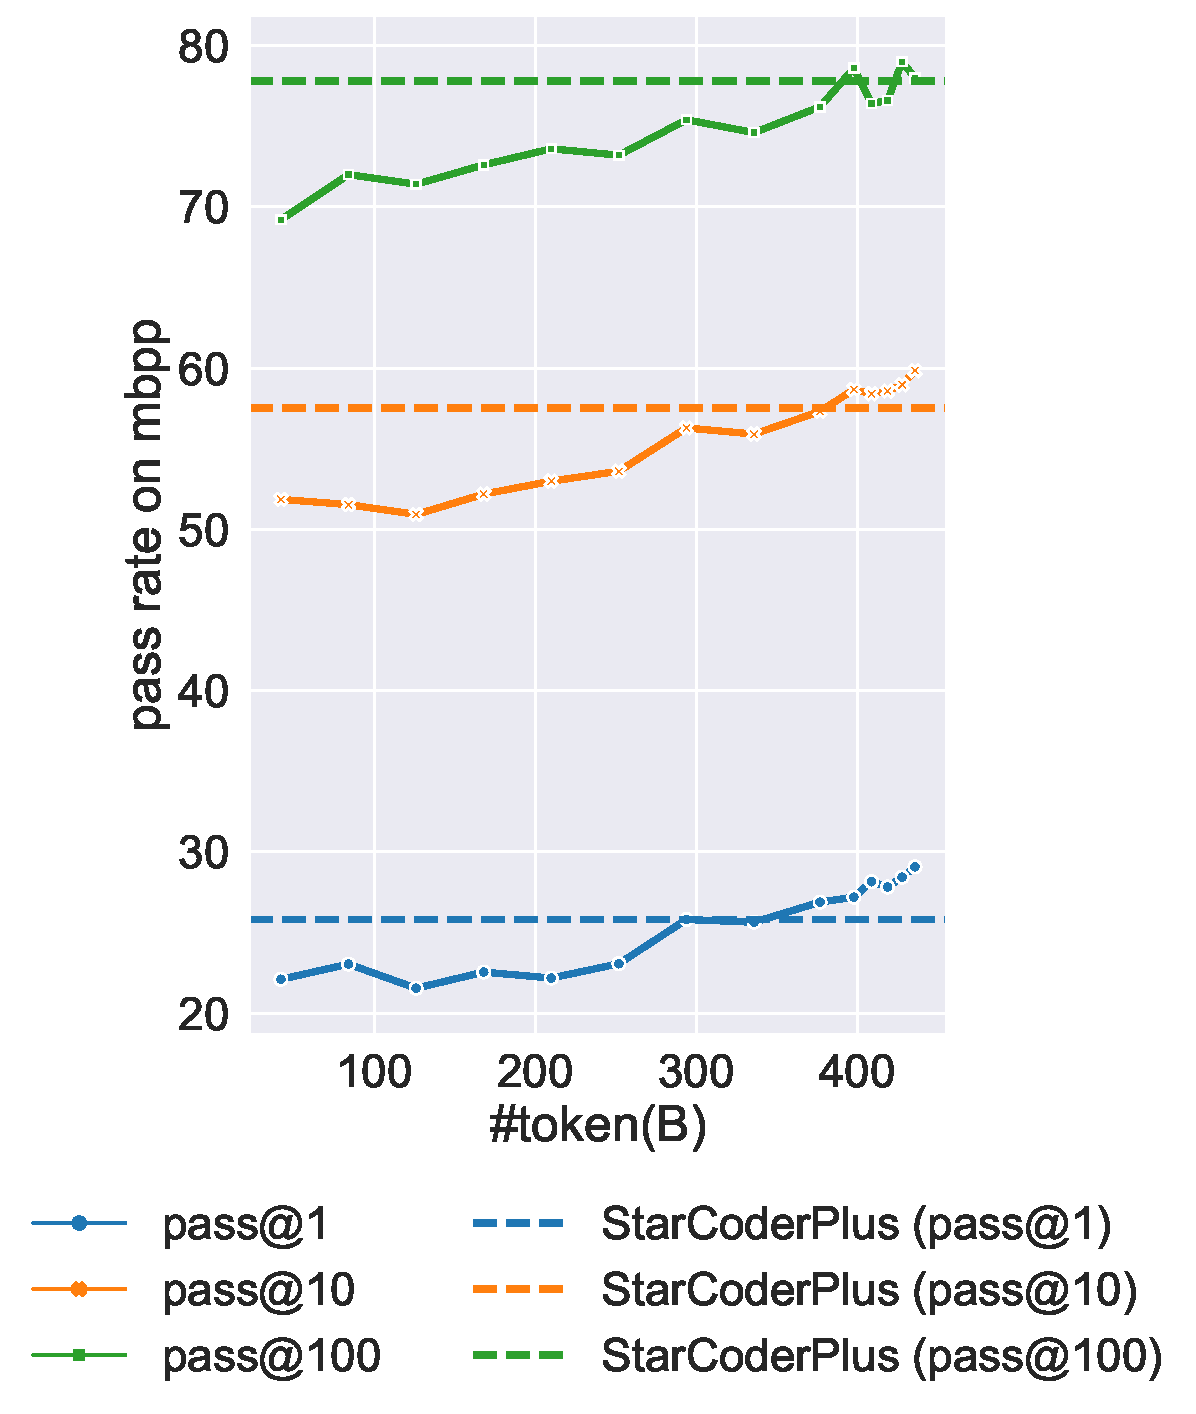
\includegraphics[width=\textwidth]{fig/mbpp-aurora-m.pdf}
        \vspace{0.42em}
        \caption{MBPP}
        \label{fig:trend-mbpp}
    \end{subfigure}
    \hfill
    \begin{subfigure}{0.33\textwidth}
        \centering
        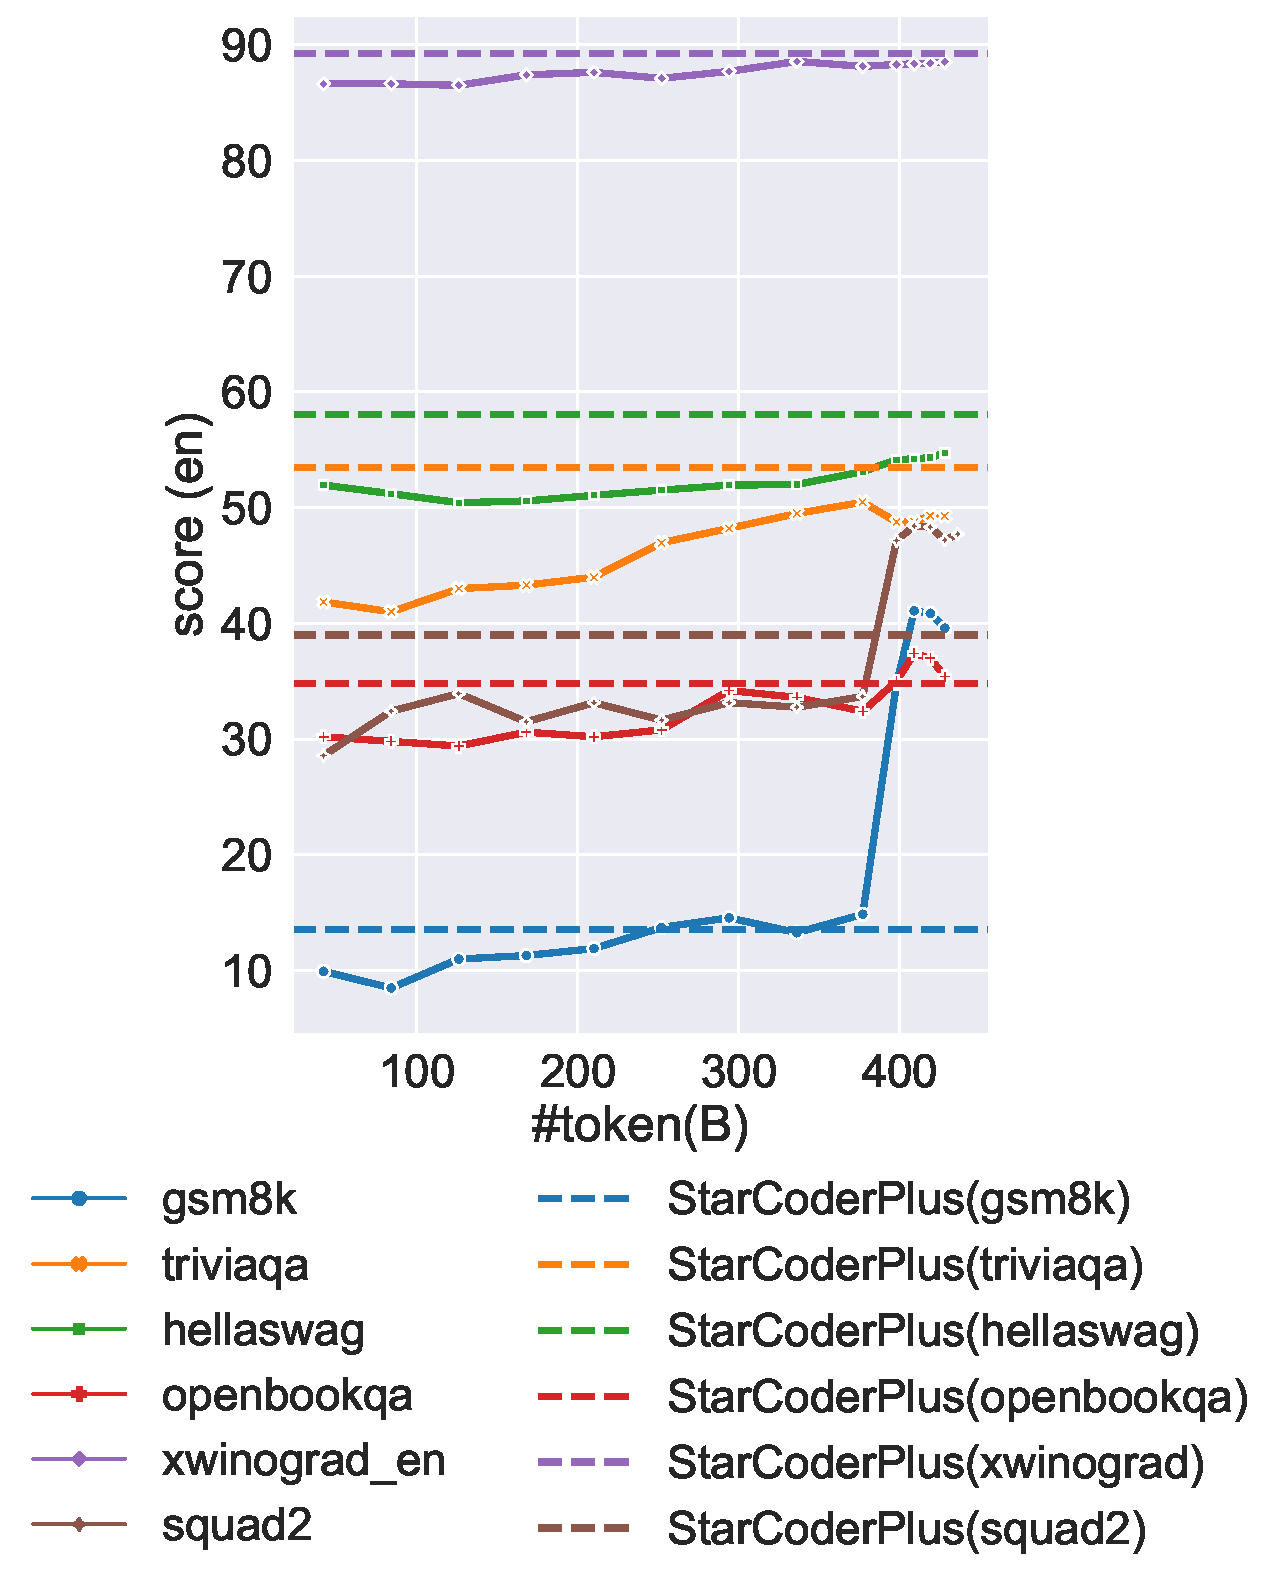
\includegraphics[width=\textwidth]{fig/aurora-m-en-fixed-optimal.pdf}
        \caption{English}
        \label{fig:trend-en}
    \end{subfigure}
    \caption{Performance trends of models on HumanEval, MBPP, and English language tasks.}
    \label{fig:ana-code-en}
\end{figure*}

\begin{figure*}[t]
    \centering
    \begin{subfigure}{0.2\textwidth}
        \centering
        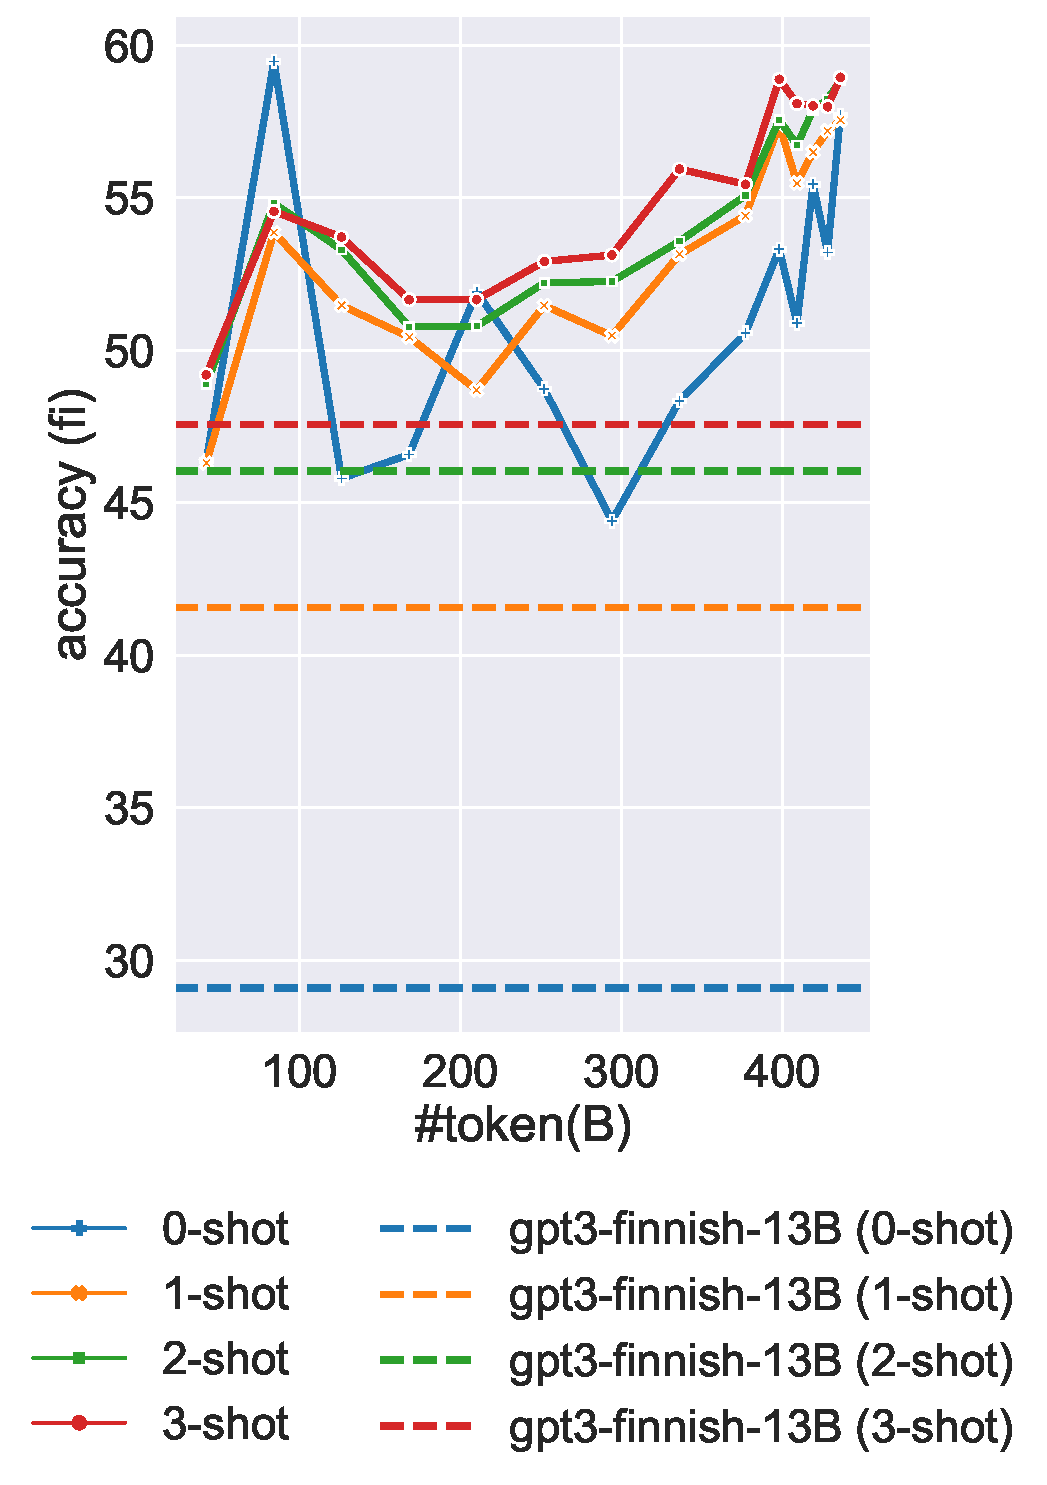
\includegraphics[width=\textwidth]{fig/aurora-m-fi.pdf}
        % \vspace{0.1em}
        \caption{Finnish}
         \label{fig:trend-fi}
    \end{subfigure}
       \hfill
    \begin{subfigure}{0.24\textwidth}
        \centering
        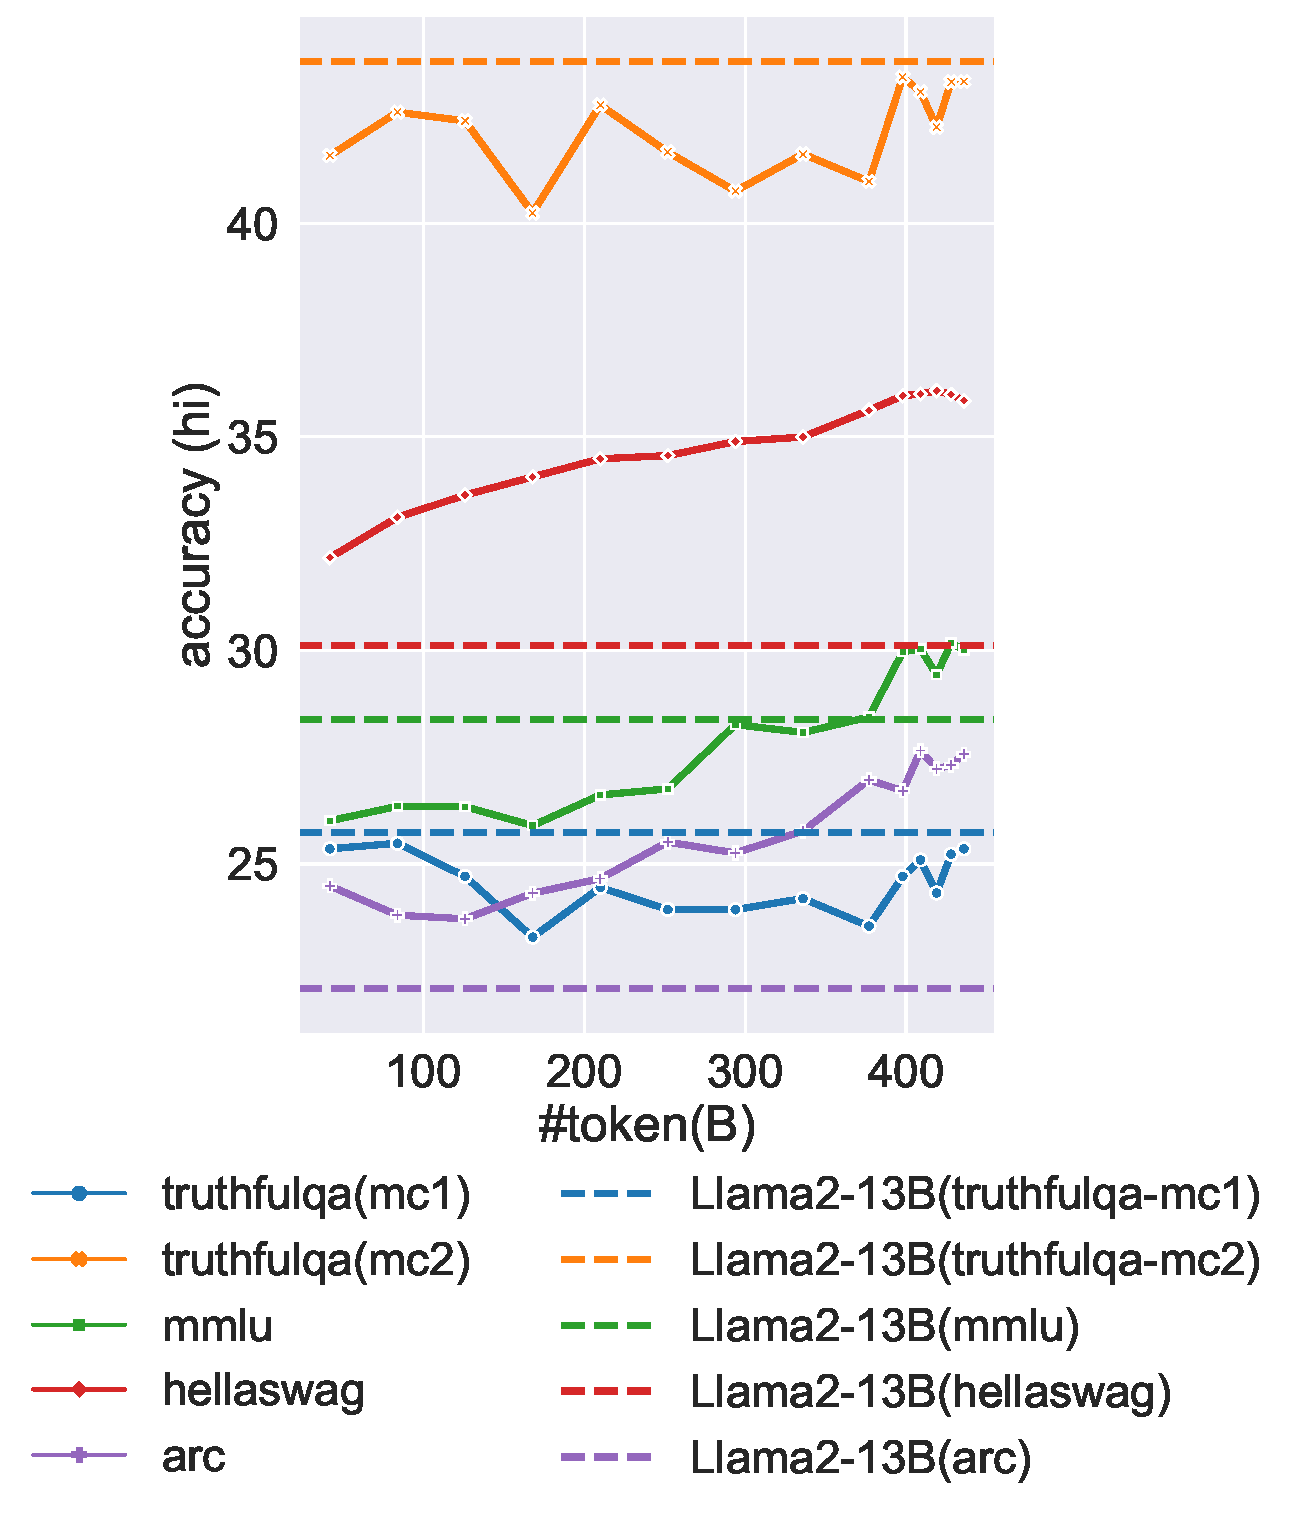
\includegraphics[width=\textwidth]{fig/aurora-m-hi.pdf}
        % \vspace{0.05em}
        \caption{Hindi}
        \label{fig:trend-hi}
    \end{subfigure}
    % \hfill
    \begin{subfigure}{0.24\textwidth}
        \centering
        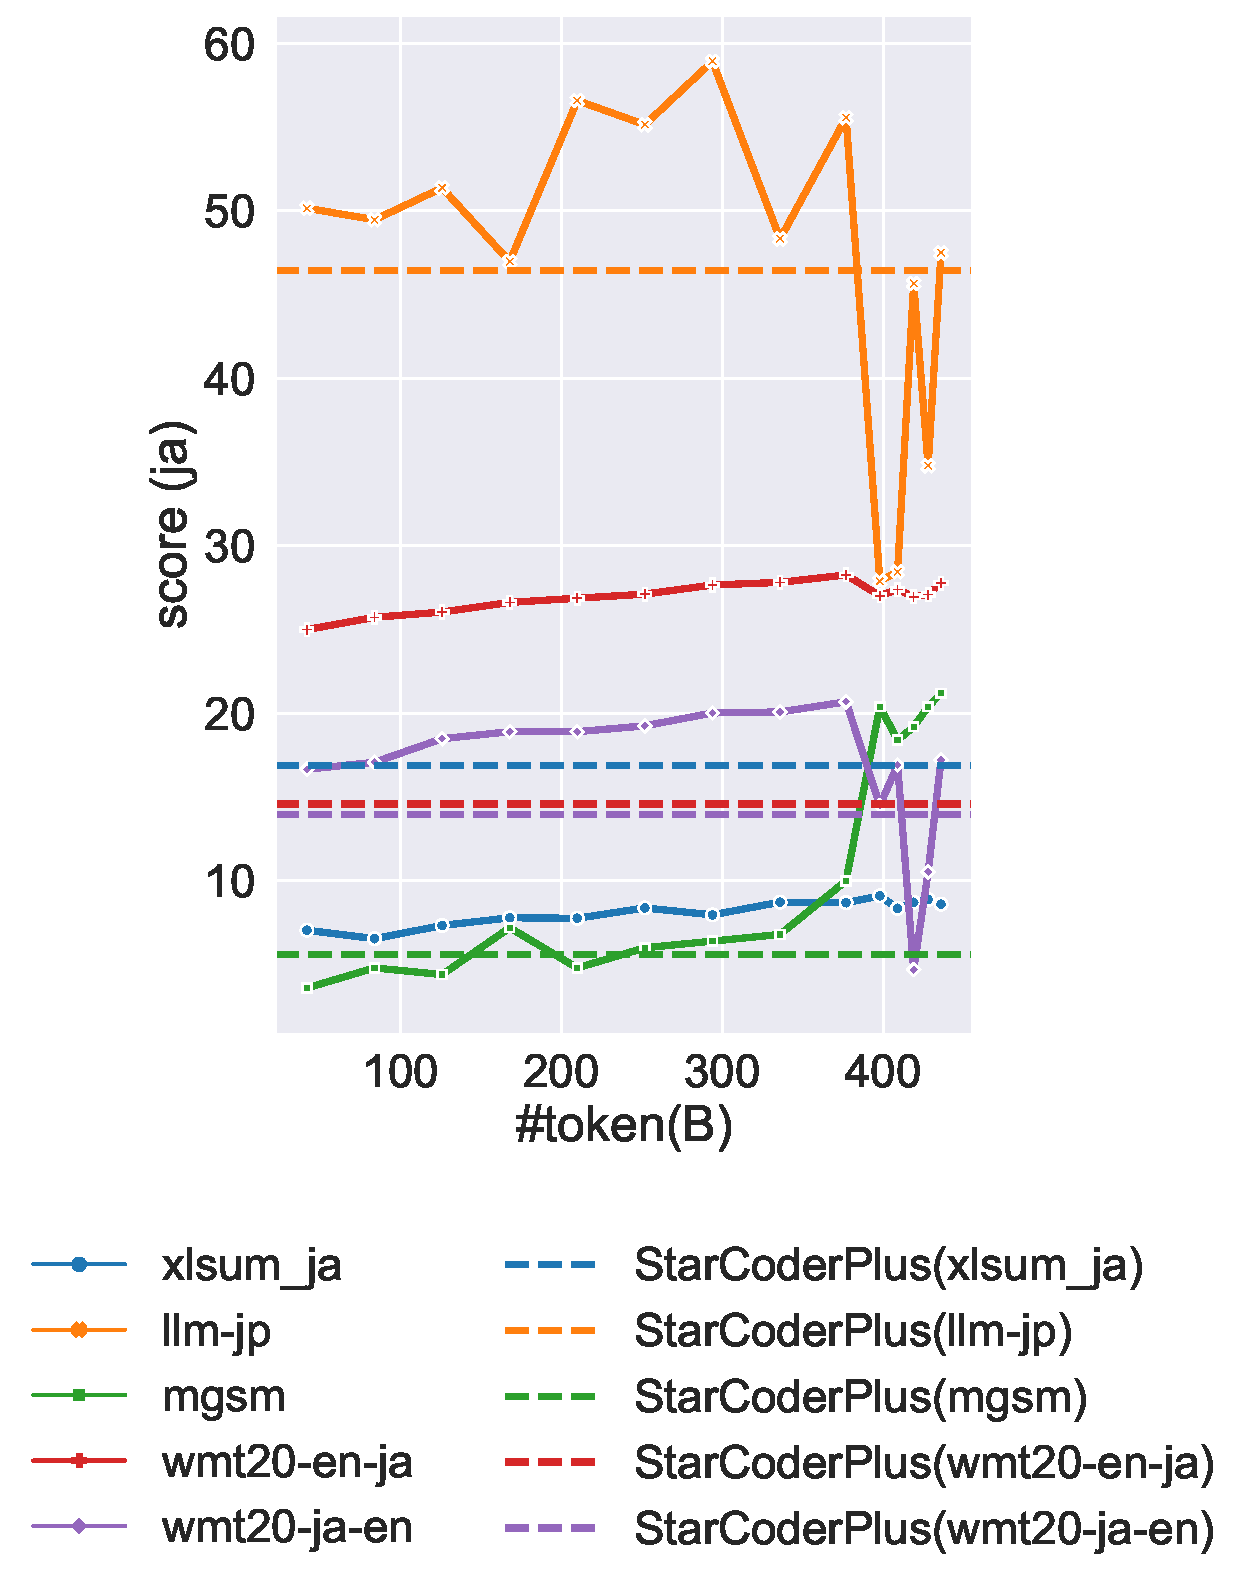
\includegraphics[width=\textwidth]{fig/aurora-m-ja.pdf}
        \caption{Japanese}
         \label{fig:trend-ja}
    \end{subfigure}
        \hfill
    \begin{subfigure}{0.24\textwidth}
        \centering
        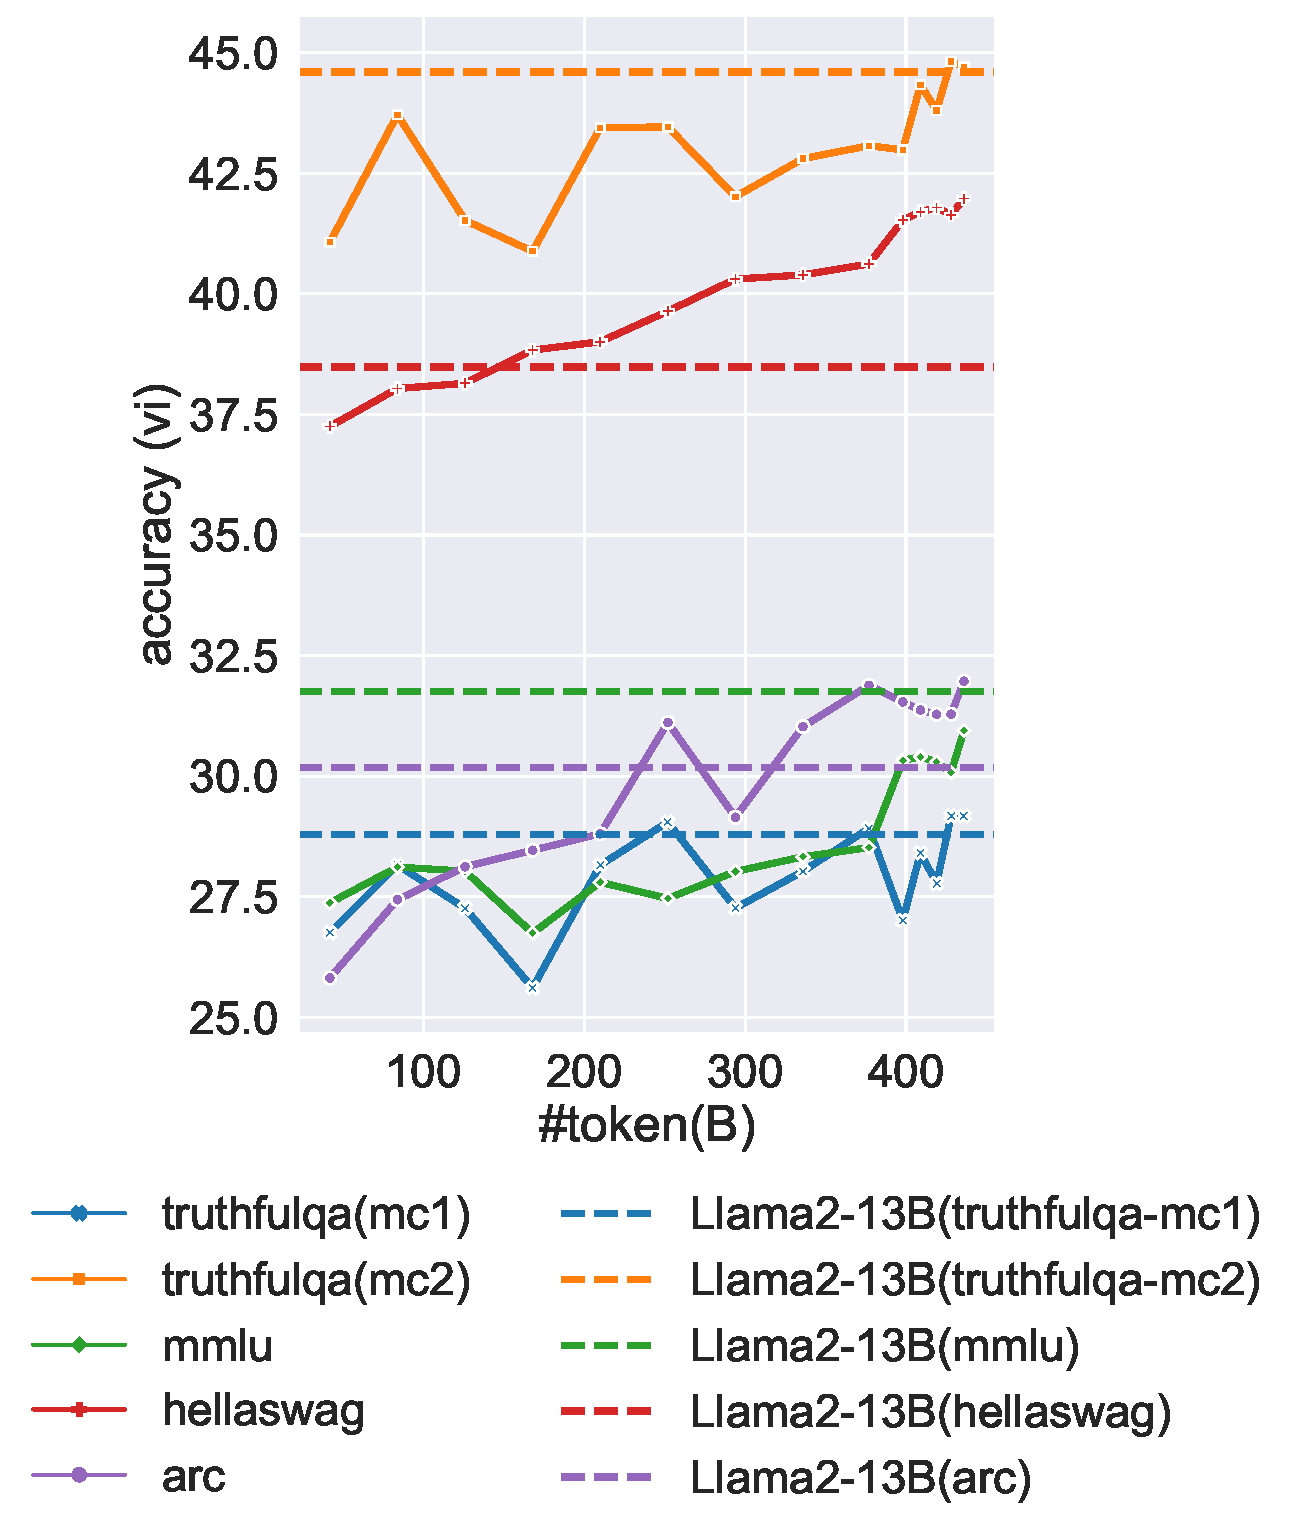
\includegraphics[width=\textwidth]{fig/aurora-m-vi.pdf}
        %\vspace{0.001em}
        \caption{Vietnamese}
         \label{fig:trend-vi}
    \end{subfigure}
    \caption{Language-specific performance trends with increasing training tokens. Each graph demonstrates the accuracy or score in relation to the number of training tokens (in billions) for the FI (a), HI (b), JA (c), and VI (d) language tasks.}
    \label{fig:ana-lg}
\end{figure*}

% \begin{figure}[thb]
%     \centering
%         \centering
%         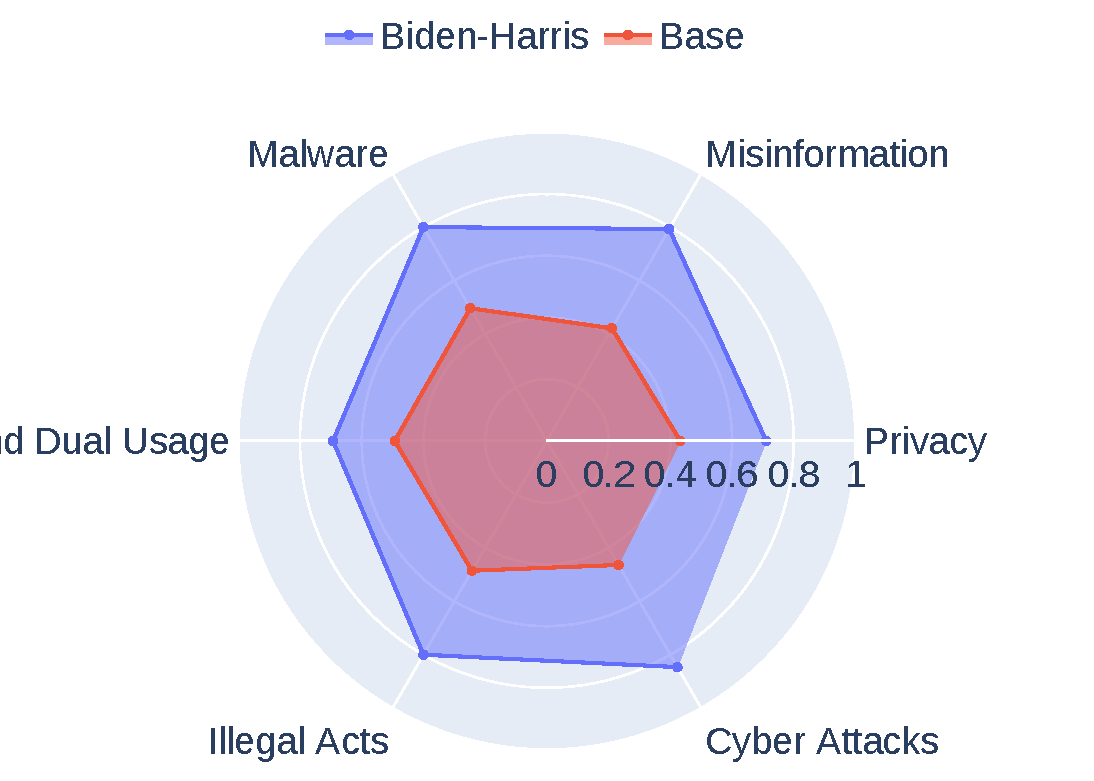
\includegraphics[width=10cm,
%   height=6cm,
%   keepaspectratio,]{fig/bh_plot_cat-1.pdf}
%         \caption{Biden-Harris Redteam Testset results, averaged over the dataset's languages by category.}\label{fig:safety_redteam}
% \end{figure}

\paragraph{Additional Safety Evaluations}\label{app:dangerous_qa}
Figure~\ref{fig:safety_dangerous} demonstrates our results on the DangerousQA dataset. Figure~\ref{fig:safety_redteam} shows the CARP values improving for our red-teamed \system. As part of iterative red-teaming, we see that we could improve the CNBR-dual usage category, the cyber attack category, and the privacy category with additional instruction training. 

\paragraph{Redteam Volunteers Protocol} Five of the authors volunteered to review and edit the generated responses from \system\ to create a subset of the Biden-Harris Redteam dataset, by editing for Biden-Harris concern violations and hateful, toxic, or bias output. One of the original volunteers and three other authors also provided CARP scores for \system\ responses to the Biden-Harris Redteam Testset shown in Figure~\ref{fig:safety_redteam}. Each volunteer is a machine learning professional over 18 years old and was informed of the risk of the sensitive subject matter of the responses.  Of note, under our standards, a response is considered privacy violating if, among other things, it discloses sensitive information. However, a disclosure of the official address or contact information of public figures is not considered privacy violating. 

\subsection{Performance Trends versus Training Token Compute}
\label{ap:ana}
% @yekun 
Figure \ref{fig:ana-code-en} and \ref{fig:ana-lg} show on the relationship between the number of training tokens and the performance of the various models. This analysis aims to capture these trends for the code generation tasks such as HumanEval and MBPP, as well as for the English, Finnish, Hindi, Japanese, and Vietnamese language evaluations.

Starting with the HumanEval and MBPP evaluations (Figures \ref{fig:trend-he} and \ref{fig:trend-mbpp}), it is evident that the pass rates improve as the number of tokens increases. This suggests that the models are benefiting from more extensive training data, which likely includes a richer variety of programming challenges and solutions that enhance the model's problem-solving abilities. Notably, the Pass@100 rate for HumanEval shows a pronounced increase, indicating that, given enough attempts, the model has a high probability of generating a correct solution. This is consistent with the iterative nature of programming, where developers often refine their code through multiple iterations.

In the English language task (Figure \ref{fig:trend-en}), there is a marked variance in performance across different tasks as the number of tokens increases. The performance on GSM8K suddenly increases, which is attributed to the effect of the instruction tuning of our second training stage (CAT). Meanwhile, TriviaQA and Hellaswag tasks show steady improvements, indicating that these tasks may be benefiting more from the increased volume of training data.


The evaluations of the Finnish (FI) (Figure \ref{fig:trend-fi}), Hindi (HI) (Figure \ref{fig:trend-hi}), Japanese (JA) (Figure \ref{fig:trend-ja}), and Vietnamese (VI) (Figure \ref{fig:trend-vi}) languages reveal a similar trend of performance improvement with the increase in the number of tokens. However, there are some variances that might be attributed to the specific challenges each language presents, such as syntactic and semantic complexities. For instance, in the Finnish graph, the performance across different shot settings indicates that the model's ability to generalize from few examples improves with more data, which is a desirable trait in language models.

The evaluations for Japanese and Vietnamese exhibit an overall positive trajectory, albeit with intermittent fluctuations. These patterns suggest the potential for sustained incremental improvement through further continual pretraining on such datasets. However, due to computational
constraints, the extended pretraining is left for future work.

